\chapter{Data Collection: The Heat Pump Dryer} \label{sec:heatpumpcollection}

\section{Purpose}

The literature review identified that the inputs to the Digital Twin Platform would be sensor data from the lower-level data collection software, and the outputs would be results from  the simulations performed by the platform. To be able to test our processes, input data was required, so a Heat Pump Dryer was chosen.

A Heat Pump Dryer provides a good test case for live data processing. Heat Pumps are a common unit operation in chemical plants. A heat pump models most thermodynamic operations, including heat exchangers, compressors, and expansion valves, including the effects of phase changes. The inclusion of a refrigerant loop makes it a good test case as recycle processes are common in industry. Gathering data from the heat pump dryer will provide some insights into the challenges involved in real-time data collection.

Since the Heat Pump Dryer includes its own control system, it does not provide a test case for closed-loop control. This is out of scope and will be a future area of research.

\begin{figure}
    \centering
    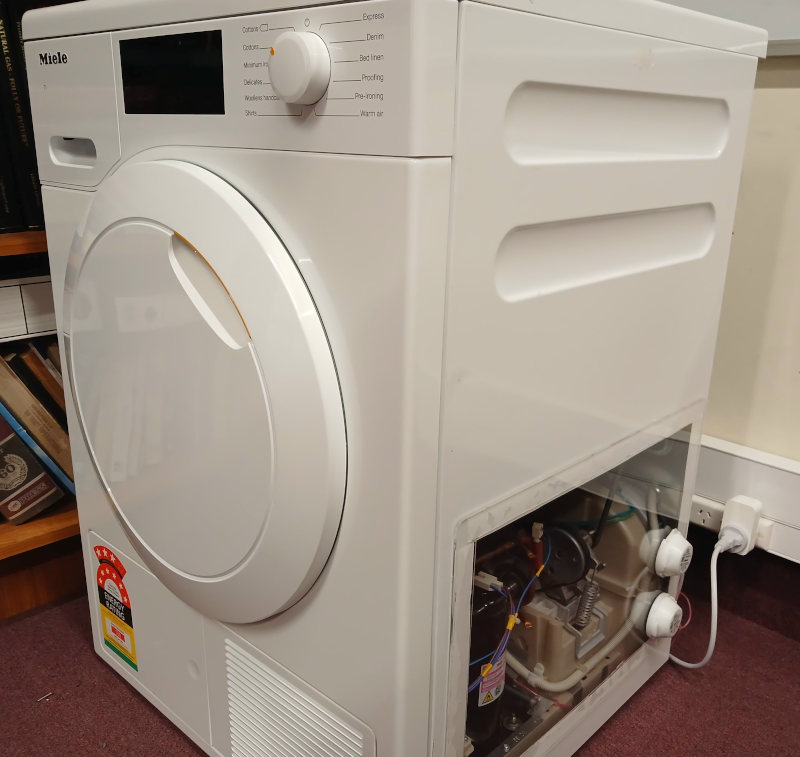
\includegraphics[width=0.4\textwidth]{dryer.png}
    \caption{Heat Pump Dryer}
    \label{fig:dryer}
\end{figure}

\section{Method}


To gather data from the heat pump dryer, Bluetooth sensors were used to measure temperature and humidity at various points in the dryer. A power meter was used to measure the total power consumption of the heat pump dryer. A raspberry pi was used to collect the data from the sensors, and store it in a InfluxDB time-series database. InfluxDB was chosen because it is one of the platforms identified in the Literature Review as being used for aggregating sensor data; it is also open-source and easy to use. This can represent the data collection system that would be used in industry.


\begin{figure}
    \centering
    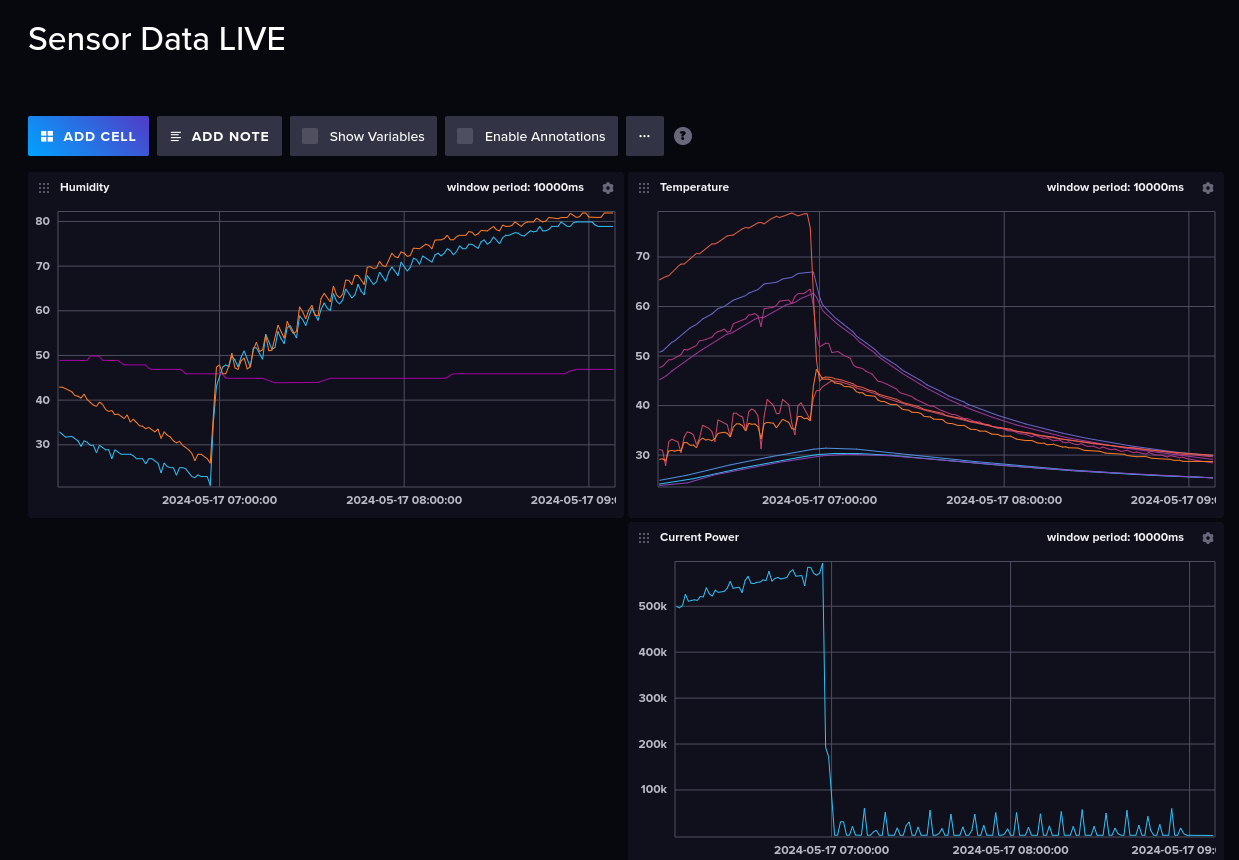
\includegraphics[width=\textwidth]{influxdb.png}
    \caption{InfluxDB Database}
    \label{fig:influxdb}
\end{figure}

\section{Insights}

The process of gathering and aggregating data was relatively straightforward. This reinforces the finding from the literature review that there are a number of tools already available for collecting and processing sensor data. 

Depending on the process, there is often only a limited amount of information that can be gleaned from the system. For example, we were not able to collect pressure information, as pressure sensors are more costly and require modification of the refrigerant loop. Likewise, we were only able to measure the total power consumption of the heat pump dryer, rather than the power consumption of individual components. Data processing techniques will need to be able to infer the state of the system from the limited data available.

Additionally, in operation, the heat pump dryer has a number of different operating cycles: it does not just continuously run all of the time: sometimes it switches direction, etc. This changes the state of the system, so the simulation will need to be able to account for this. We did not have access to the control system of the heat pump dryer, so we were unable to collect data on the operating cycles. Depending on the setup in industry, this data may or may not be avaliable.
